	\documentclass[10pt,oneside]{CBFT_book}
	% Algunos paquetes
	\usepackage{amssymb}
	\usepackage{amsmath}
	\usepackage{graphicx}
	\usepackage{libertine}
	\usepackage[bold-style=TeX]{unicode-math}
	\usepackage{lipsum}

	\usepackage{natbib}
	\setcitestyle{square}

	\usepackage{polyglossia}
	\setdefaultlanguage{spanish}


	\usepackage{CBFT.estilo} % Cargo la hoja de estilo

	% Tipografías
	% \setromanfont[Mapping=tex-text]{Linux Libertine O}
	% \setsansfont[Mapping=tex-text]{DejaVu Sans}
	% \setmonofont[Mapping=tex-text]{DejaVu Sans Mono}

	%===================================================================
	%	DOCUMENTO PROPIAMENTE DICHO
	%===================================================================

\begin{document}

% =================================================================================================
\chapter{Expansión en un campo multipolar}
% =================================================================================================


\begin{figure}[htb]
	\begin{center}
	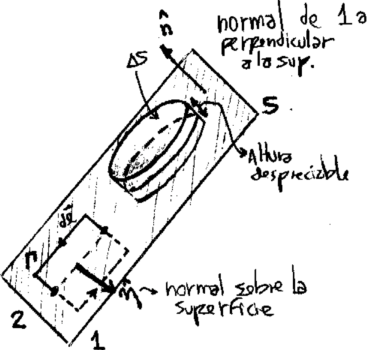
\includegraphics[width=0.6\textwidth]{images/fig_ft1_contorno1.pdf}	 
	\end{center}
	\caption{}
\end{figure} 

\begin{figure}[htb]
	\begin{center}
	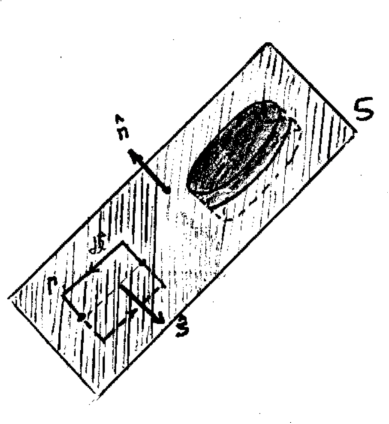
\includegraphics[width=0.6\textwidth]{images/fig_ft1_contorno2.pdf}	 
	\end{center}
	\caption{}
\end{figure} 

% =================================================================================================
\section{Desarrollo multipolar}
% =================================================================================================



\begin{figure}[htb]
	\begin{center}
	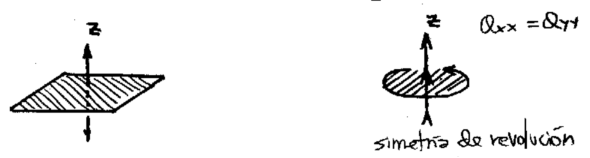
\includegraphics[width=0.6\textwidth]{images/fig_ft1_multipolo2.pdf}	 
	\end{center}
	\caption{}
\end{figure}

\begin{figure}[htb]
	\begin{center}
	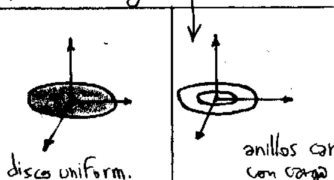
\includegraphics[width=0.6\textwidth]{images/fig_ft1_multipolo3.pdf}	 
	\end{center}
	\caption{}
\end{figure}

\begin{figure}[htb]
	\begin{center}
	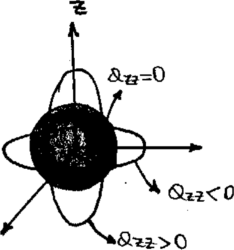
\includegraphics[width=0.6\textwidth]{images/fig_ft1_multipolo4.pdf}	 
	\end{center}
	\caption{}
\end{figure}


% =================================================================================================
\section{Dipolo}
% =================================================================================================

\begin{figure}[htb]
	\begin{center}
	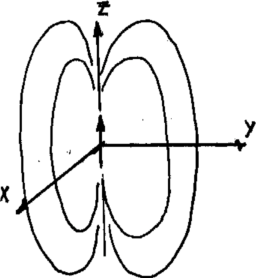
\includegraphics[width=0.6\textwidth]{images/fig_ft1_dipolar2.pdf}	 
	\end{center}
	\caption{}
\end{figure}

\begin{figure}[htb]
	\begin{center}
	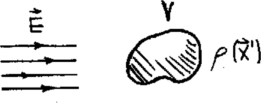
\includegraphics[width=0.6\textwidth]{images/fig_ft1_dipolar3.pdf}	 
	\end{center}
	\caption{}
\end{figure}


\begin{figure}[htb]
	\begin{center}
	\includegraphics[width=0.6\textwidth]{images/fig_dipolarvol.pdf}	 
	\end{center}
	\caption{}
\end{figure} 


% =================================================================================================
\section{Campo dipolar}
% =================================================================================================

\begin{figure}[htb]
	\begin{center}
	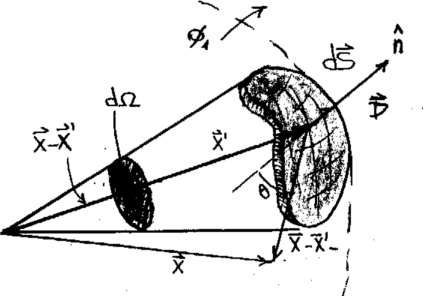
\includegraphics[width=0.6\textwidth]{images/fig_ft1_campo_dipolar1.pdf}	 
	\end{center}
	\caption{}
\end{figure}

\begin{figure}[htb]
	\begin{center}
	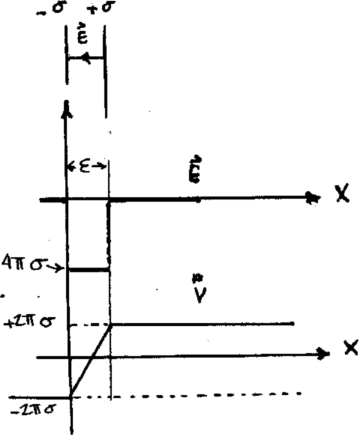
\includegraphics[width=0.6\textwidth]{images/fig_ft1_campo_dipolar2.pdf}	 
	\end{center}
	\caption{}
\end{figure}

\begin{figure}[htb]
	\begin{center}
	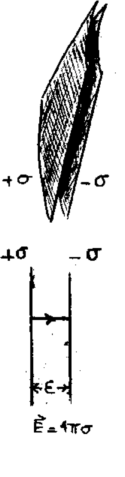
\includegraphics[width=0.6\textwidth]{images/fig_ft1_campo_dipolar3.pdf}	 
	\end{center}
	\caption{}
\end{figure}







% \bibliographystyle{CBFT-apa-good}	% (uses file "apa-good.bst")
% \bibliography{CBFT.Referencias} % La base de datos bibliográfica

\end{document}
